\documentclass[12pt,a4paper,oneside]{report}

% VIT SCOPE project-report layout, implemented in XeLaTeX.
\usepackage[a4paper,top=4cm,bottom=3cm,left=4.5cm,right=2.5cm]{geometry}
\usepackage{fontspec}
\setmainfont{Times New Roman}
\setmonofont{Menlo}[Scale=0.82]
\usepackage{amsmath,amssymb,mathtools}
\usepackage{setspace}
\onehalfspacing
\usepackage{microtype}
\usepackage{graphicx}
\usepackage{booktabs,longtable,tabularx,array,multirow}
\usepackage{enumitem}
\setlist{itemsep=2pt,topsep=4pt,leftmargin=1.7em}
\usepackage{listings}
\usepackage{tikz}
\usetikzlibrary{arrows.meta,positioning,shapes.geometric,fit,calc}
\usepackage{caption}
\usepackage{titlesec}
\usepackage{fancyhdr}
\usepackage{hyperref}
\usepackage{xurl}
\usepackage{float}
\usepackage{makecell}
\usepackage{chngcntr}
\hypersetup{colorlinks=false,pdfborder={0 0 0},pdftitle={Design and Implementation of a CLR Parser Generator},pdfauthor={Gurutheja Kavuturi; Ephraim Immanuel I; Goyal Hemant Anil; Raymond Dhakal}}
\urlstyle{same}
\setlength{\parindent}{1.2em}
\setlength{\parskip}{0pt}
\setlength{\headheight}{15pt}
\renewcommand{\headrulewidth}{0pt}
\fancyhf{}
\fancyhead[R]{\thepage}
\pagestyle{fancy}
\fancypagestyle{plain}{\fancyhf{}\fancyhead[R]{\thepage}\renewcommand{\headrulewidth}{0pt}}
\titleformat{\chapter}[display]{\bfseries\centering\fontsize{14}{18}\selectfont}{CHAPTER \thechapter}{8pt}{\MakeUppercase}
\titlespacing*{\chapter}{0pt}{0pt}{24pt}
\titleformat{\section}{\bfseries\fontsize{14}{18}\selectfont}{\thesection}{0.8em}{}
\titleformat{\subsection}{\bfseries\fontsize{14}{18}\selectfont}{\thesubsection}{0.8em}{}
\titleformat{\subsubsection}{\bfseries\fontsize{12}{15}\selectfont}{\thesubsubsection}{0.8em}{}
\counterwithin{figure}{chapter}
\counterwithin{table}{chapter}
\renewcommand{\figurename}{Fig.}
\captionsetup[figure]{position=bottom,justification=centering,font=small,labelfont=bf}
\captionsetup[table]{position=top,justification=raggedright,singlelinecheck=false,font=small,labelfont=bf}
\setcounter{secnumdepth}{3}
\setcounter{tocdepth}{2}
\newcommand{\code}[1]{\texttt{\detokenize{#1}}}
\newcommand{\filepath}[1]{\path{#1}}
\newcommand{\term}[1]{\textit{#1}}
\newcommand{\placeholderline}{\rule{0.34\textwidth}{0.4pt}}
\lstdefinestyle{source}{basicstyle=\ttfamily\small,breaklines=true,columns=fullflexible,keepspaces=true,frame=single,rulecolor=\color{black!45},showstringspaces=false,captionpos=b,aboveskip=8pt,belowskip=8pt}
\lstset{style=source}
\newcolumntype{Y}{>{\raggedright\arraybackslash}X}
\newcommand{\chapterintro}[1]{\noindent\textbf{Chapter overview.} #1\par\vspace{8pt}}
\newcommand{\stage}[3]{\textbf{#1} & #2 & #3\\}

\begin{document}
\pagenumbering{roman}
\thispagestyle{empty}
\begin{titlepage}
\centering
\vspace*{0.15cm}

\includegraphics[width=0.62\textwidth]{assets/vit-logo.jpeg}\par
\vspace{0.35cm}
{\bfseries\large SCHOOL OF COMPUTER SCIENCE AND ENGINEERING (SCOPE)\par}
\vspace{0.25cm}
{\bfseries BCSE307L COMPILER DESIGN\par}
\vspace{0.65cm}
{\bfseries\fontsize{17}{21}\selectfont DESIGN AND IMPLEMENTATION OF A CLR PARSER GENERATOR USING CANONICAL LR(1) ITEM SETS, LOOKAHEAD PROPAGATION, CLOSURE-GOTO CONSTRUCTION AND CONFLICT ANALYSIS\par}
\vspace{0.55cm}
{\large Extended with the Leo Programming Language Compiler and Browser Playground\par}
\vspace{1cm}
A project report submitted in partial fulfillment of the requirements for the course\par
\vspace{0.25cm}
{\bfseries BCSE307L Compiler Design\par}
\vspace{0.9cm}
{\bfseries Team Members\par}
\vspace{0.2cm}
\begin{tabular}{ll}
Gurutheja Kavuturi & 24BEL0086\\
Ephraim Immanuel I & 24BEL0091\\
Goyal Hemant Anil & 24BYB0059\\
Raymond Dhakal & 24BEL0100\\
\end{tabular}\par
\vspace{0.4cm}
Under the guidance of\par
{\bfseries Prof. Vishnu Priya A\par}
\vspace{0.15cm}
October 2026\par
\end{titlepage}

\chapter*{DECLARATION}
\addcontentsline{toc}{chapter}{Declaration}
We, the undersigned members of the project team, submit this report titled \emph{Design and Implementation of a CLR Parser Generator Using Canonical LR(1) Item Sets, Lookahead Propagation, Closure-GOTO Construction and Conflict Analysis}. It describes the design and implementation of the team's Canonical LR(1) parser generator and its extension into the Leo programming-language compiler. The report distinguishes the project implementation from established compiler theory and identifies the external sources used for theoretical background.\par
\vspace{0.7cm}
The technical descriptions and implementation figures are attributed to the project repository or review material from which they were obtained. Where those records report different parser-state or test totals, this report identifies the figures by source and time rather than presenting them as one comparable run. The project test suite was not rerun solely for preparation of this report.\par
\vspace{1cm}
\begin{tabularx}{\textwidth}{>{\centering\arraybackslash}X >{\centering\arraybackslash}X}
\placeholderline & \placeholderline\\
Gurutheja Kavuturi & Ephraim Immanuel I\\
24BEL0086 & 24BEL0091\\[1.1cm]
\placeholderline & \placeholderline\\
Goyal Hemant Anil & Raymond Dhakal\\
24BYB0059 & 24BEL0100\\
\end{tabularx}
\vfill
\textbf{Place:} Vellore \hfill \textbf{Date:} \placeholderline
\clearpage

\chapter*{BONAFIDE CERTIFICATE}
\addcontentsline{toc}{chapter}{Bonafide Certificate}
This is to certify that the project report entitled \emph{Design and Implementation of a CLR Parser Generator Using Canonical LR(1) Item Sets, Lookahead Propagation, Closure-GOTO Construction and Conflict Analysis} is a record of the project work carried out by Gurutheja Kavuturi (24BEL0086), Ephraim Immanuel I (24BEL0091), Goyal Hemant Anil (24BYB0059), and Raymond Dhakal (24BEL0100), submitted in partial fulfillment of the requirements of BCSE307L Compiler Design at the School of Computer Science and Engineering, Vellore Institute of Technology, Vellore.\par
\vspace{0.6cm}
The report documents the construction of a Canonical LR(1) parser generator and its application in a six-phase compiler for Leo. This certificate page is provided in the department's report format and is intended for completion and signature by the authorized faculty and examiners.\par
\vspace{2.3cm}
\begin{tabularx}{\textwidth}{>{\centering\arraybackslash}X >{\centering\arraybackslash}X}
\placeholderline & \placeholderline\\
Prof. Vishnu Priya A & Internal Examiner\\
Faculty In-Charge / Guide & Name and Signature\\[1.7cm]
\placeholderline & \placeholderline\\
External Examiner & Head of School / Authorized Signatory\\
Name and Signature & Name and Signature\\
\end{tabularx}
\vfill
School of Computer Science and Engineering (SCOPE)\\
Vellore Institute of Technology, Vellore, India
\clearpage

\chapter*{ACKNOWLEDGEMENT}
\addcontentsline{toc}{chapter}{Acknowledgement}
The project brought together formal-language theory, systems programming, compiler construction, and iterative software development. We thank Prof. Vishnu Priya A, Faculty In-Charge for BCSE307L Compiler Design, for providing the academic setting in which the work was developed and reviewed. We also acknowledge the School of Computer Science and Engineering and Vellore Institute of Technology for the course structure and facilities supporting the project.\par
\vspace{0.35cm}
We thank the members of the team for implementing and integrating the grammar engine, FIRST-set computation, LR(1) items, closure and GOTO operations, canonical collection, parsing tables, conflict analysis, parser driver, compiler phases, and browser interface. The modular design made it possible to test the parser generator independently before connecting it to a programming-language front end.\par
\vspace{0.35cm}
We are grateful to the authors of the compiler-design literature cited in this report. Their published explanations of LR parsing, syntax-directed translation, intermediate representations, and data-flow analysis provide the theoretical foundation against which the implementation can be understood. We also acknowledge the maintainers of the tools and libraries used to build and serve the compiler demonstration.\par
\vspace{0.35cm}
Finally, we thank classmates and reviewers who tried the grammar examples and Leo playground and reported confusing behavior. Their feedback helped us improve error messages, clarify the language reference, and separate the command-line compiler, browser playground, and project-question interface in the documentation.
\vfill
\begin{flushright}
The Project Team\\
Vellore, October 2026
\end{flushright}
\clearpage

\tableofcontents
\clearpage
\listoftables
\addcontentsline{toc}{chapter}{List of Tables}
\clearpage
\listoffigures
\addcontentsline{toc}{chapter}{List of Figures}
\clearpage

\chapter*{LIST OF ABBREVIATIONS}
\addcontentsline{toc}{chapter}{List of Abbreviations}
\begin{longtable}{p{0.22\textwidth}p{0.70\textwidth}}
\toprule
\textbf{Abbreviation} & \textbf{Expansion}\\
\midrule
AST & Abstract Syntax Tree\\
CFG & Control-Flow Graph\\
CLR(1) & Canonical LR parser with one lookahead terminal\\
DFA & Deterministic Finite Automaton\\
FIRST & Set of terminals that can begin strings derived from a symbol or sequence\\
GCC & GNU Compiler Collection\\
GOTO & Parser-state transition induced by a grammar symbol\\
IR & Intermediate Representation\\
LR & Left-to-right scan, rightmost derivation in reverse\\
RAG & Retrieval-Augmented Generation\\
SLR(1) & Simple LR parser with one lookahead terminal\\
WASI & WebAssembly System Interface\\
WASM & WebAssembly\\
\bottomrule
\end{longtable}
\clearpage

\chapter*{NOMENCLATURE}
\addcontentsline{toc}{chapter}{Nomenclature}
\begin{longtable}{p{0.22\textwidth}p{0.70\textwidth}}
\toprule
\textbf{Notation} & \textbf{Meaning in this report}\\
\midrule
$G=(N,T,P,S)$ & Context-free grammar with non-terminals $N$, terminals $T$, productions $P$, and start symbol $S$.\\
$S'$ & Fresh augmented start symbol.\\
$A\to\alpha$ & Production with left-hand side $A$ and right-hand side $\alpha$.\\
$[A\to\alpha\cdot\beta,a]$ & LR(1) item with dot position and terminal lookahead $a$.\\
$\epsilon$ & Empty string.\\
$\$$ & End-of-input terminal used by the parser.\\
$\mathrm{FIRST}(\beta a)$ & Terminals that can begin a derivation of $\beta a$.\\
$\mathrm{CLOSURE}(I)$ & Items implied by an item set $I$ and LR(1) lookahead propagation.\\
$\mathrm{GOTO}(I,X)$ & Closed set reached by advancing over grammar symbol $X$.\\
$C$ & Canonical collection of LR(1) item sets.\\
$\mathrm{ACTION}[i,a]$ & Shift, reduce, accept, or error action for state $i$ and terminal $a$.\\
$\mathrm{GOTO}[i,A]$ & State transition for state $i$ and non-terminal $A$.\\
\bottomrule
\end{longtable}
\clearpage

\chapter*{ABSTRACT}
\addcontentsline{toc}{chapter}{Abstract}
Compiler construction joins formal grammars with executable systems. This project implements a Canonical LR(1) parser generator in C and then uses the generator as the syntax-analysis core of Leo, a small imperative programming language and six-phase compiler. The generator reads a whitespace-tokenized context-free grammar, augments its start production, computes nullability and FIRST sets, propagates terminal lookaheads through closure, constructs GOTO transitions and the complete canonical collection, builds ACTION and GOTO tables, detects shift-reduce and reduce-reduce conflicts, and drives a table-based shift-reduce parser. The parser is not generated from fixed language-specific tables: the compiler loads Leo's grammar at startup and builds its states and tables from that grammar.\par
\vspace{0.3cm}
The compiler extends this core through lexical analysis, CLR(1) parsing with abstract-syntax-tree construction, scoped semantic analysis, three-address intermediate code, control-flow-graph optimization, and C code generation. A command-line driver can emit C and invoke GCC, or execute intermediate code in an interpreter. The Leo language includes integer, floating-point, and Boolean types; declarations and assignments; conditional and loop statements; input; and two print forms. The source tree also includes a static browser playground. In that facility, a WebAssembly build runs in a Web Worker through a WASI shim, presents compiler-phase outputs, and interprets the program's intermediate code in the browser. A separate project-question interface indexes selected project documentation and source text locally, retrieves relevant passages, and uses Groq for answer generation. The question-answering interface is an auxiliary documentation feature rather than part of the compiler pipeline.\par
\vspace{0.3cm}
The design emphasizes explicit lookahead propagation, deterministic conflict reporting, phase boundaries, source-position diagnostics, and repeatable tests. Current repository documentation records 856 canonical states and no conflicts for the Leo grammar, and 500 passing tests. The attached Review Stage 2 slides contain earlier figures of 391 states and 298 tests; those figures are retained as historical review results, not combined with the newer repository record. A fresh build and test run is required to reconcile the records before final submission. The report describes the algorithms, data flow, implementation modules, test strategy, limitations, and future extensions, with established compiler theory cited separately from the project-specific implementation.

\clearpage
\pagenumbering{arabic}
\setcounter{page}{1}
\chapter{INTRODUCTION}
\chapterintro{This chapter defines the project problem, explains why the team built a parser generator before a full compiler, and states the objectives and boundaries of the Leo implementation.}

\section{Background}
A compiler translates a program written in one language into a form that can be executed by a target machine or runtime. Its work is commonly divided into front-end analysis, intermediate representations, optimization, and target-code generation. Each stage has a different responsibility: recognizing character sequences, checking whether tokens form grammatical structures, checking meaning and types, and lowering the validated program into an executable representation. A project that implements these stages can therefore make compiler concepts concrete and expose how information changes as it passes through the system [2].

Parsing is a central boundary in this pipeline. A lexer classifies character groups as tokens, but a parser determines how those tokens combine according to a grammar. A parser generator makes this relationship explicit: the grammar is input data, and the generator constructs a state machine and parsing table from it. In this project, the chosen construction is full Canonical LR(1), also called CLR(1), where an item contains a production position and one terminal lookahead. The generator is useful on its own for arbitrary grammars in the project's text format and is also used by Leo's compiler.

The project grew from a standalone parser-generator implementation into a larger compiler. This extension made the generator's behavior observable on a real programming language rather than only on small expression grammars. It also required semantic hooks in the parser so reductions could construct an abstract syntax tree without replacing the original shift-reduce driver.

\section{Problem Definition}
The project addresses two connected problems. First, implement a parser generator that accepts a context-free grammar and constructs a canonical LR(1) parser, including its full item sets, transitions, action tables, and conflict report. Second, use that generator in a compiler for Leo, taking Leo source through lexical, syntactic, semantic, intermediate-code, optimization, and C-generation phases.

The standalone generator must correctly propagate lookaheads through nullable suffixes, preserve distinct states whose LR(0) cores match but lookaheads differ, and report table collisions instead of silently overwriting an action. The compiler must map every grammar terminal to a lexer token, provide a semantic action for each production used to build the AST, reject invalid types and scopes, preserve source locations for diagnostics, and stop after the first failed phase. The project also needs command-line and browser interfaces that let a reader inspect intermediate results.

\section{Motivation}
A manually written parser can recognize a language, but its relationship to the grammar may be difficult to audit. A grammar-driven generator makes production rules, lookaheads, state transitions, and parse decisions inspectable. That property is especially helpful in a compiler-design course, where the implementation should demonstrate not only that example programs work but also how the parsing table was obtained.

Choosing canonical LR(1) emphasizes lookahead precision. SLR(1) reductions use FOLLOW sets, which are global to a non-terminal; LALR(1) merges states that share cores; canonical LR(1) retains the lookahead context on each item and does not merge distinct lookahead states. The cost is a potentially larger state collection. This project accepts that cost for a small language so that the construction can be studied directly [1], [2].

The second motivation is integration. A standalone parser demonstrates table construction but does not show how parsing interacts with a lexer, an AST, type checking, optimization, or code generation. Leo gives the generator an end-to-end use while keeping the parser algorithm general.

\section{Aim and Objectives}
The aim is to design and implement a Canonical LR(1) parser generator and use it as the parsing foundation of a six-phase compiler for Leo.

The objectives are:
\begin{enumerate}
  \item Represent terminals, non-terminals, productions, LR(1) items, item sets, transitions, actions, conflicts, and tables in reusable C data structures.
  \item Compute nullable symbols and FIRST sets by fixed-point iteration.
  \item Implement LR(1) CLOSURE using $\mathrm{FIRST}(\beta a)$ and implement GOTO by advancing the dot and closing the result.
  \item Enumerate the canonical collection and build the ACTION and GOTO tables from state transitions and completed items.
  \item Detect and explain shift-reduce and reduce-reduce conflicts, and refuse to compile a grammar with unresolved conflicts.
  \item Implement a table-driven parser with tracing and expected-token diagnostics.
  \item Extend the parser with reduction hooks that construct Leo's AST, and connect it to semantic analysis, IR, optimization, and C generation.
  \item Provide CLI and browser access to the compiler and document the implementation and its evidence.
\end{enumerate}

\section{Scope and Boundaries}
The generator supports context-free grammars expressed as whitespace-separated symbols, alternatives, an explicit start directive, and an epsilon marker. It does not transform grammars automatically, recover after syntax errors, or compress canonical states into LALR states. The input grammar is used as written, and a conflict is treated as a compile-time grammar failure.

Leo is a small, statically checked imperative language. Its documented features include INT, FLOAT, and BOOL; declarations; assignments; conditional statements; WHILE, REPEAT-UNTIL, and FOR loops; INPUT; PRINT; and PRINTN. It has no arrays or functions, and strings are limited to print items and input prompts. The native back end emits C and invokes GCC. The web build executes the IR interpreter rather than spawning a native C compiler in the browser.

The RAG question interface is included as a documentation aid. It does not participate in tokenization, parsing, optimization, or program execution. It retrieves selected project passages and submits those passages with a question to Groq; the key is kept on the server. It is treated as a related interface, not as evidence that the compiler requires an LLM.

\section{Project Contributions}
The project contributions can be grouped into four parts. The first is a reusable Canonical LR(1) construction in C, from grammar loading through conflict analysis and table-driven parsing. The second is the integration of this core into an extensible programming-language front end using parser hooks to build an AST. The third is a complete small-language pipeline that lowers to three-address code, optimizes that representation, emits C, and optionally interprets the IR. The fourth is the set of demonstrations and engineering material around the implementation: a command-line driver, test suite, language specification, browser playground, and local project-question interface.

These contributions should not be confused with the underlying LR theory, which predates this project and is cited in the literature review. The project contribution is an implementation and integration of these established ideas, including its data structures, code paths, diagnostics, tests, and interfaces.

\section{Report Organization}
Chapter 2 reviews compiler and LR-parsing literature and identifies the design choices made here. Chapter 3 presents the proposed system and its boundaries. Chapter 4 develops the requirements, algorithms, architecture, and data structures. Chapter 5 describes implementation details by module and by compiler phase. Chapter 6 presents the available test evidence and discusses what it does and does not establish. Chapter 7 concludes with limitations and future work. The appendices provide a Leo example, algorithm summaries, a test-case catalogue, and operational instructions.

\chapter{LITERATURE SURVEY}
\chapterintro{This chapter separates standard compiler theory from the team's implementation choices. It surveys canonical LR parsing, compiler phase organization, intermediate representations, and the role of systematic testing.}

\section{Compiler Construction}
Compiler design is usually explained as a sequence of analyses and transformations. A front end reads source text, reports lexical and syntactic errors, builds a representation of program structure, and checks language-level constraints. A middle end can transform a machine-independent intermediate representation. A back end maps the validated representation to target code and runtime support [2]. The separation does not require every implementation to use the same number of phases; it gives each phase a well-defined input and output.

The six-phase organization in Leo makes these boundaries visible. Lexical analysis produces tokens. Syntax analysis consumes those tokens and creates an AST. Semantic analysis annotates and validates the AST with types and symbol information. IR generation lowers structured statements to instructions and labels. Optimization transforms the IR under language-specific safety rules. Code generation emits C, after which GCC performs native compilation. This is a project-specific phase decomposition that follows the broader compiler architecture described in standard texts [2].

\section{LR Parsing and Canonical Lookahead}
Knuth's work formalized LR(k) grammars and bottom-up parsing with bounded lookahead [1]. The LR notation describes a left-to-right scan and a rightmost derivation in reverse. An LR parser uses a stack and a state-dependent action table to choose whether to shift an input terminal, reduce a recognized handle, accept, or report an error.

An LR(1) item augments a production with a dot and a lookahead terminal. For example, $[A\to\alpha\cdot B\beta,a]$ records that the parser has recognized $\alpha$, expects a derivation beginning with $B\beta$, and may reduce in a context associated with lookahead $a$. The dot is not an input character; it is a compact representation of parser progress through a production.

Canonical LR(1) construction starts from an augmented start production and computes a closure for each state. When the dot precedes a non-terminal, productions of that non-terminal are introduced with lookaheads from $\mathrm{FIRST}(\beta a)$. The suffix $\beta$ matters: if it can derive the empty string, the original lookahead $a$ can follow the newly expanded non-terminal. The generator therefore needs nullability and FIRST-set support, not only a direct copy of the current lookahead.

\section{SLR, LALR, and CLR Design Trade-offs}
SLR(1), LALR(1), and canonical LR(1) all use shift-reduce parsing, but differ in how they construct states and reduction lookaheads. SLR(1) uses LR(0) cores with FOLLOW sets for reductions. That compact strategy may assign a reduction in a context where the canonical item would have a narrower terminal lookahead. LALR(1) begins with canonical LR(1) states and merges states with equal LR(0) cores, combining their lookahead sets. This often reduces table size, but a merge can introduce conflicts that were absent before. Canonical LR(1) retains the full state distinctions and thus gives the most direct representation of one-token contexts among the three approaches [2].

The project deliberately implements canonical LR(1), not because it is always the smallest or fastest parser, but because full lookahead propagation is the principal subject of the parser-generator work. The generated grammar for Leo is modest enough for rebuilding the canonical collection at startup. The implementation does not claim that canonical state construction is the best choice for every production compiler.

\begin{table}[H]
\centering
\caption{High-Level Comparison of LR Table Construction Choices}
\begin{tabularx}{\textwidth}{p{2.0cm}YYY}
\toprule
\textbf{Method} & \textbf{State basis} & \textbf{Reduction context} & \textbf{Project relevance}\\
\midrule
SLR(1) & LR(0) item sets & FOLLOW sets & Smaller baseline, but not the selected lookahead method.\\
LALR(1) & Merged canonical cores & Union of lookaheads for merged states & A possible future compression stage, not implemented.\\
CLR(1) & Full LR(1) item sets & Item-specific terminal lookahead & Implemented method; preserves canonical contexts and exposes lookahead propagation.\\
\bottomrule
\end{tabularx}
\end{table}

\section{Grammar Transformations and Precedence}
A parser generator consumes a grammar; the grammar designer remains responsible for expressing the language's structure. One common approach is to specify operator precedence and associativity through separate declarations. Another is to use a hierarchy of non-terminals so that each level represents a precedence class. Leo uses the second approach: OR, AND, equality, relation, addition/subtraction, multiplication/division, power, unary operators, and primary expressions are layered in the grammar.

This construction makes associativity visible in productions. Left-recursive rules such as $AddExpr\to AddExpr + MulExpr$ encode left association; the power rule uses a right-recursive form to encode right association. Because precedence is structural, the generator does not need a separate precedence resolver to break parse-table conflicts. The project grammar consequently builds without conflicts in the current repository record.

\section{Syntax-Directed Translation and Semantic Hooks}
A parser can do more than accept or reject a token sequence. A reduction identifies a production whose right-hand side has been recognized. A semantic action associated with that reduction can build an AST node from the semantic values of the right-hand-side symbols. This style of syntax-directed translation is a standard compiler technique [2].

The project adds optional parser hooks for shift, reduce, and discard events while keeping the standalone parser behavior and trace available. Each stack entry can carry a semantic value. Leo's parser binds semantic actions to production text and constructs AST nodes at reductions. The compiler checks that every terminal is associated with a lexer token and that each grammar production has an action; a mismatch is reported as a grammar integration error rather than causing a later null or malformed node.

\section{Intermediate Representations and Optimization}
An intermediate representation separates source syntax from target code. Three-address instructions name a destination and at most a small number of operands, while labels and conditional jumps describe control flow. The representation used by Leo is typed and includes explicit input/output operations, arithmetic and Boolean operations, branches, labels, and jumps.

Optimization then works on this representation. The implemented optimizer forms basic blocks and a control-flow graph, propagates constants with a finite lattice, applies safe algebraic identities, propagates local copies, removes unreachable branches, and performs liveness-based dead-code removal. The transformation rules are constrained by Leo's semantics: potentially failing division, MOD, and negative integer exponentiation are not removed or evaluated early. Floating-point identities that do not preserve NaN or signed-zero behavior are also excluded. These are project decisions built on general data-flow ideas [2].

\section{Survey Summary and Design Gap}
The literature establishes the theory of canonical LR parsing and the organization of compiler phases. The implementation gap addressed by the project is educational and integrative: a learner should be able to follow the grammar through FIRST sets, item closure, state transitions, ACTION/GOTO construction, conflict checking, reductions, AST construction, type analysis, IR, optimization, and generated C in one repository.

The parser-generator component is generic with respect to its grammar format. The compiler component supplies Leo's grammar and semantic actions. The browser playground exposes intermediate phases to make behavior inspectable. No claim is made that these features improve on mature industrial parser generators in throughput, memory use, or language coverage. The report evaluates the implementation against its own scope and test evidence.

\chapter{OVERVIEW OF THE PROPOSED SYSTEM}
\chapterintro{This chapter describes the project as a set of related but distinct tools: a general CLR(1) generator, the Leo compiler, a browser playground, and a documentation question-answering service.}

\section{System Context}
The main system receives either a grammar and token string for the standalone parser generator, or a Leo source file for the compiler. In the compiler path, the grammar is loaded at startup and used to build parsing tables. The lexer reads the source program and emits tokens with source positions. The parser feeds those tokens through the canonical table and creates an AST. Later compiler phases consume the AST rather than re-parsing source text.

The system has two execution paths after code generation. In a terminal build, the driver writes C source and can invoke GCC using process creation and an argument vector. In interpreter mode, the optimized IR is executed directly. The browser build uses the same compiler logic compiled to WebAssembly, but runs its interpreter because a browser worker cannot invoke a host GCC process.

\begin{figure}[H]
\centering
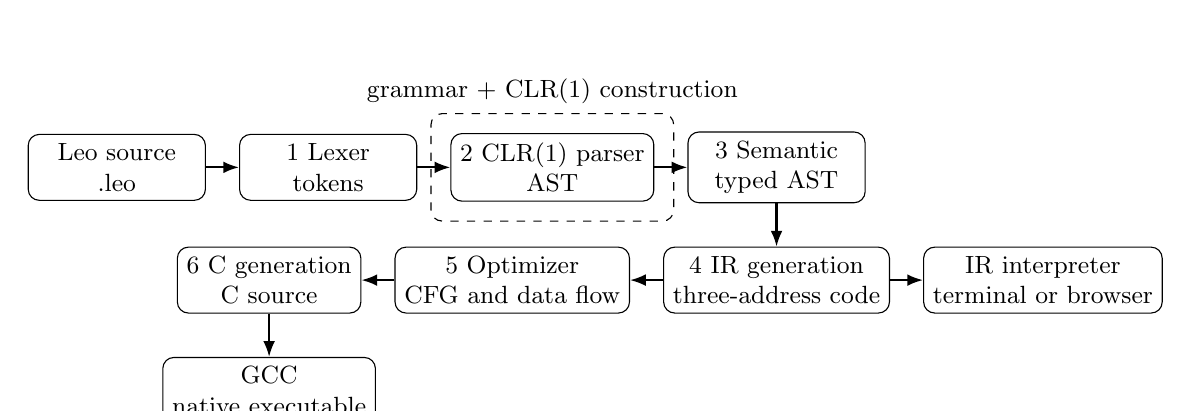
\begin{tikzpicture}[node distance=0.55cm and 0.42cm, box/.style={draw,rounded corners,align=center,minimum width=2.25cm,minimum height=0.8cm,font=\small}, arr/.style={-{Latex[length=2mm]},thick}]
\node[box] (src) {Leo source\\.leo};
\node[box,right=of src] (lex) {1 Lexer\\tokens};
\node[box,right=of lex] (parse) {2 CLR(1) parser\\AST};
\node[box,right=of parse] (sem) {3 Semantic\\typed AST};
\node[box,below=of sem] (ir) {4 IR generation\\three-address code};
\node[box,left=of ir] (opt) {5 Optimizer\\CFG and data flow};
\node[box,left=of opt] (cg) {6 C generation\\C source};
\node[box,below=of cg] (gcc) {GCC\\native executable};
\node[box,right=of ir] (interp) {IR interpreter\\terminal or browser};
\draw[arr] (src)--(lex); \draw[arr] (lex)--(parse); \draw[arr] (parse)--(sem);
\draw[arr] (sem)--(ir); \draw[arr] (ir)--(opt); \draw[arr] (opt)--(cg);
\draw[arr] (cg)--(gcc); \draw[arr] (ir)--(interp);
\node[draw,dashed,rounded corners,fit=(parse),inner sep=7pt,label=above:{\small grammar + CLR(1) construction}] {};
\end{tikzpicture}
\caption{Six-Phase Leo Compiler Pipeline and Execution Options}
\label{fig:pipeline}
\end{figure}

\section{Standalone Parser Generator}
The standalone tool reads a grammar file in the documented token format. A grammar line identifies a left-hand side, an arrow, and one or more right-hand-side alternatives. Symbols are whitespace-separated. A symbol occurring as a production left-hand side is a non-terminal; other symbols are terminals. The start symbol is declared explicitly, and the generator adds a fresh augmented production. The special epsilon marker represents an empty right-hand side, while the end marker is reserved for parser operation.

The standalone driver can display the parsed grammar, FIRST sets, canonical states, table entries, conflicts, and parse trace. A user can supply a whitespace-separated token sequence to test a grammar. Its value is not limited to Leo: test grammars include simple, expression, epsilon, and intentionally conflicting examples.

\section{Leo Programming Language}
Leo is designed to be small enough for a course compiler while containing enough constructs to exercise the pipeline. Types are INT, FLOAT, and BOOL. Statements include declarations, assignments, IF with optional ELSE, WHILE, REPEAT-UNTIL, FOR, INPUT, PRINT, and PRINTN. Assignment uses \code{<-}; subtraction and unary negation use \code{~}. Comments begin with \code{#}.

PRINT writes its items without a trailing newline, while PRINTN ends the line and can be used without items for a blank line. Input can be read directly or preceded by a prompt. Integer variables use a 64-bit representation and wrap according to the emitted C compilation settings; FLOAT uses double precision; BOOL is represented by an integer and printed symbolically. Only INT widens implicitly to FLOAT. Conditions must be Boolean. The full specification is in \code{language/language_spec.md}.

\section{Browser Playground}
The static playground presents an editor, examples, a pre-run input box, an output view, and tabs for tokens, AST, IR, optimized IR, and generated C. The browser loads the WebAssembly compiler in a Web Worker through a WASI shim. This keeps compilation work away from the main UI thread. Section markers in the compiler output let the page split one run into phase-specific panels.

The interactive input path can resume a Leo program when INPUT requests data. A run is restarted in the deterministic interpreter with the values collected so far, so the browser experience reproduces the same result without retaining a suspended native stack. The Playground is a teaching interface and does not execute emitted C in the browser. A user can download the .leo source and inspect or download generated C.

\section{Project Question Interface}
A second web page answers questions about project files. The indexer extracts eligible text from documentation, source, headers, and web assets into a local chunk index. At request time, retrieval ranks passages for a question. The backend sends the question and selected excerpts to Groq using a server-side API key, and the model generates a response grounded in those excerpts. The frontend displays the answer and file/line sources.

This path uses an LLM; the compiler and playground do not. The RAG service is read-only with respect to project files, and retrieved material is context for an answer rather than executable input to the compiler. The server does not intentionally send the entire repository: it sends the question and the retrieved chunks. As the configured provider is external, the operator should understand that the selected excerpts and question leave the local machine for answer generation.

\begin{table}[H]
\centering
\caption{Project Components and Their Responsibilities}
\begin{tabularx}{\textwidth}{p{2.8cm}p{3.4cm}Y}
\toprule
\textbf{Component} & \textbf{Input} & \textbf{Output / responsibility}\\
\midrule
CLR(1) generator & Grammar text and token stream & FIRST sets, canonical states, ACTION/GOTO tables, conflict report, parse result.\\
Leo compiler & .leo source and optional input & Diagnostics, phase outputs, IR, C source, executable or interpreter output.\\
Browser playground & Source, example, user input & Interactive compiler-phase display using WebAssembly and IR interpretation.\\
RAG indexer & Selected project files & Local text chunks with source locations.\\
RAG server & Question, retrieved chunks, Groq configuration & Grounded answer with citations to project paths and lines.\\
\bottomrule
\end{tabularx}
\end{table}

\section{Users and Operational Scenarios}
A compiler-design student can run the standalone generator on a tiny grammar, inspect the item sets, and compare the state transitions with the grammar. A Leo programmer can compile a file, request only the AST or IR, emit C, or run the interpreter. A reviewer can use the browser playground to try examples and inspect intermediate output without installing a native compiler toolchain. A project teammate can use the question interface to locate relevant implementation details in the repository.

These scenarios share source material but have different trust and execution boundaries. The CLI accepts a file path and may invoke GCC only when a build mode requires it. The browser has no shell access and runs the interpreter in WASM. The RAG service reads the local index and calls a remote model API; it does not invoke the compiler or alter source files.

\chapter{PROPOSED SYSTEM ANALYSIS AND DESIGN}
\chapterintro{This chapter turns the project objectives into functional requirements, describes the principal algorithms and structures, and records the constraints that shape the implementation.}

\section{Requirement Analysis}
The requirements are divided into functional behavior and quality constraints. Functional requirements describe observable operations. Non-functional requirements cover clarity, portability, reliability, and predictable behavior. The project is a course-scale implementation, so the requirements focus on correctness within the defined grammar and language rather than industrial throughput or broad language compatibility.

\subsection{Functional Requirements}
\begin{longtable}{p{1.5cm}p{0.32\textwidth}p{0.53\textwidth}}
\caption{Functional Requirements for the Project}\\
\toprule
\textbf{ID} & \textbf{Requirement} & \textbf{Acceptance evidence}\\
\midrule
FR-01 & Load and validate a context-free grammar. & Grammar loader identifies symbols, productions, start symbol, and malformed input.\\
FR-02 & Compute nullability and FIRST sets. & FIRST output and grammar tests cover recursive and epsilon cases.\\
FR-03 & Build canonical LR(1) item sets. & Closure and GOTO preserve terminal lookaheads; canonical states are deduplicated.\\
FR-04 & Construct parser tables. & Terminal transitions, completed items, accept item, and non-terminal transitions populate appropriate cells.\\
FR-05 & Detect conflicts. & Shift-reduce and reduce-reduce collisions are recorded with state and lookahead.\\
FR-06 & Parse token streams. & Parser shifts, reduces, accepts, rejects, and can print a trace.\\
FR-07 & Build Leo ASTs. & Reduction hooks construct nodes and attach source positions.\\
FR-08 & Check language semantics. & Type, declaration, scope, and condition errors are reported before IR generation.\\
FR-09 & Generate and optimize IR. & Statements lower to typed three-address operations; optimizer preserves observable traps.\\
FR-10 & Emit and run target code. & C can be emitted; GCC builds an executable when requested; interpreter mode does not require GCC.\\
FR-11 & Expose compiler results in a browser. & Playground presents output and phase tabs and can request interactive input.\\
FR-12 & Answer project questions from project sources. & RAG retrieves file excerpts and returns source-linked answers through Groq.\\
\bottomrule
\end{longtable}

\subsection{Non-Functional Requirements}
\begin{itemize}
\item \textbf{Inspectability:} the generator can display grammar-derived states and tables; the compiler can expose phase artifacts.
\item \textbf{Deterministic failure:} a phase error stops later stages and maps to a defined exit status.
\item \textbf{Source safety:} generated artifacts go to an output directory; compiler output must not overwrite the input source.
\item \textbf{Portability:} the native code uses C and common process APIs; the build supports Make and CMake. The browser uses WebAssembly.
\item \textbf{Usability:} diagnostics identify source positions and expected tokens where available; examples and language documentation explain syntax.
\item \textbf{Maintainability:} modules have explicit data structures and phase boundaries, and the same parser core supports a standalone mode and semantic hooks.
\item \textbf{Security boundary:} native compiler invocation uses fork/exec with arguments rather than a shell command string; the Groq key is read by the server, not embedded in browser code.
\end{itemize}

\subsection{System Requirements}
The native compiler requires a C11 compiler, a C math library, and Make or CMake. GCC is the default target compiler for producing an executable, though C code generation and interpreter mode can be used without invoking GCC. The browser version requires a modern browser with WebAssembly, JavaScript modules, Web Workers, and HTTP hosting. The RAG backend uses Python 3, the packages listed in \code{requirements.txt}, a local project-root environment file or equivalent environment variables, and a valid Groq API key for answer generation.

\section{Grammar and Input Model}
The generator treats the grammar as a finite set of productions. It augments the start symbol with a new production so acceptance has a unique completed item. Terminal and non-terminal identities are stored as integer symbol identifiers, allowing item sets and tables to refer to symbols without copying their strings at every edge.

For a production $A\to X_1X_2\ldots X_n$, an LR(1) item records the production and dot position $i$, together with a lookahead terminal $a$. The item is commonly written $[A\to X_1\ldots X_i\cdot X_{i+1}\ldots X_n,a]$. A completed item has the dot at the end. A shift transition advances the dot over a terminal; a reduce action is considered for the item's lookahead.

\subsection{Nullable and FIRST Analysis}
A non-terminal is nullable if it derives the empty string. Initially, direct epsilon productions make their left-hand sides nullable. The fixed-point iteration then marks a left-hand side nullable when all symbols in one of its right-hand sides are nullable. For each production, FIRST accumulates the first terminals reachable from the right-hand side; the scan continues through nullable prefixes and stops at the first non-nullable symbol. If every symbol is nullable, the left-hand side is nullable too.

For an LR(1) closure item with a non-terminal after the dot, the generator must compute FIRST of the suffix followed by the existing lookahead. If $\beta$ is nullable, the terminal lookahead itself is included. The code's sequence routine accepts a trailing lookahead so this rule is applied consistently for any suffix length.

\subsection{CLOSURE Construction}
Given an item set $I$, CLOSURE starts with all members of $I$ and repeatedly examines items with a non-terminal $B$ immediately after the dot. For each production $B\to\gamma$, it adds items $[B\to\cdot\gamma,b]$ for every $b\in\mathrm{FIRST}(\beta a)$, where the original item is $[A\to\alpha\cdot B\beta,a]$. The set stops growing when a full pass introduces no new item.

The implementation uses a worklist-like pass strategy. A pass scans the items present at its start; new items are examined in the next pass. The process terminates because the grammar has finitely many productions, dot positions, and terminal lookaheads. Item equality includes the production, dot position, and lookahead, so two otherwise identical cores with distinct lookahead terminals remain distinct.

\subsection{GOTO and Canonical Collection}
For a grammar symbol $X$, GOTO of state $I$ advances the dot over $X$ in every item where $X$ appears immediately after the dot, then closes the advanced set. An empty advanced set has no transition. Reusing the closure routine avoids a second implementation of lookahead propagation.

Canonical collection construction begins with the closure of the augmented start item with end marker lookahead. A breadth-first worklist processes discovered states. For every symbol immediately after a dot in a state, it computes GOTO. If the result equals an existing complete item set, the transition points to that state; otherwise a new state is created and queued. A state comparison must compare complete LR(1) item sets, not only LR(0) cores.

\begin{figure}[H]
\centering
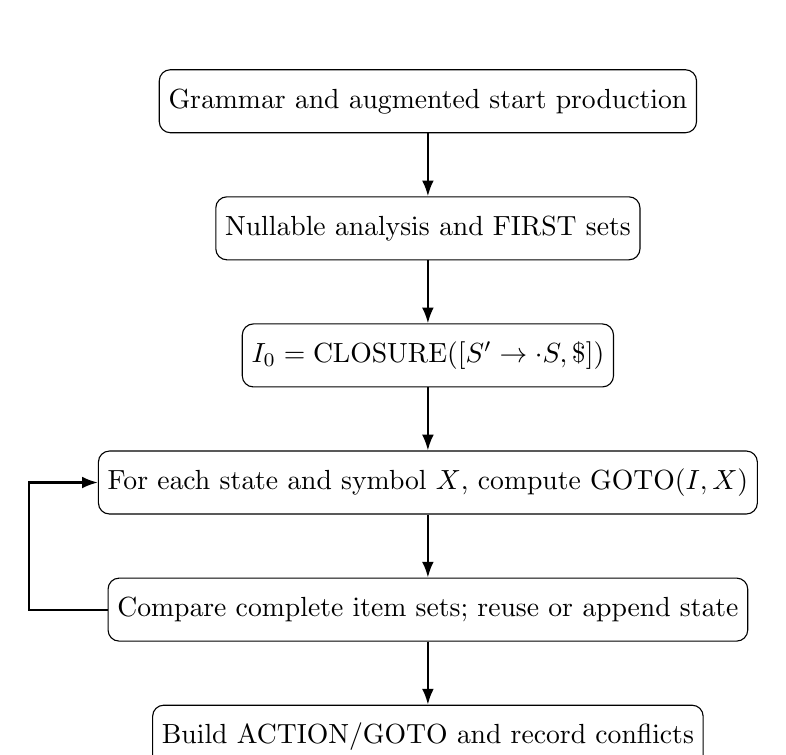
\begin{tikzpicture}[node distance=0.8cm, box/.style={draw,rounded corners,align=center,minimum width=4.2cm,minimum height=0.8cm}, arr/.style={-{Latex[length=2mm]},thick}]
\node[box] (gram) {Grammar and augmented start production};
\node[box,below=of gram] (first) {Nullable analysis and FIRST sets};
\node[box,below=of first] (start) {$I_0=\mathrm{CLOSURE}([S'\to\cdot S,\$])$};
\node[box,below=of start] (expand) {For each state and symbol $X$, compute $\mathrm{GOTO}(I,X)$};
\node[box,below=of expand] (dedup) {Compare complete item sets; reuse or append state};
\node[box,below=of dedup] (table) {Build ACTION/GOTO and record conflicts};
\draw[arr] (gram)--(first); \draw[arr] (first)--(start); \draw[arr] (start)--(expand); \draw[arr] (expand)--(dedup); \draw[arr] (dedup)--(table);
\draw[arr] (dedup.west) -- ++(-1.0,0) |- (expand.west);
\end{tikzpicture}
\caption{Canonical Collection Construction Work Flow}
\label{fig:canonical-workflow}
\end{figure}

\section{Parsing Table Design}
For every terminal transition from state $i$ to state $j$ on terminal $a$, the table receives a shift action in $\mathrm{ACTION}[i,a]$. For every completed non-augmented item $[A\to\alpha\cdot,a]$, a reduce action for $A\to\alpha$ is entered under lookahead $a$. The completed augmented item places accept under the end marker. A transition on a non-terminal $A$ is stored in $\mathrm{GOTO}[i,A]$.

The table builder detects attempts to assign incompatible actions to one cell. The first action is retained in the data structure and the attempted collision is appended to a conflict list with the state, lookahead, and competing actions. Retaining the first value ensures the table remains representable for diagnostics; it does not mean the grammar is accepted. The compiler refuses to proceed when conflicts exist.

\section{Shift-Reduce Parser}
The parser maintains a state stack and a symbol stack. The top state and next input terminal select an action. A shift pushes the terminal and destination state and advances the input. A reduce action removes the right-hand-side length from the stacks, identifies the left-hand-side non-terminal, consults GOTO from the exposed state, and pushes the reduced symbol and state. The parser accepts only when the table selects accept. A missing action reports a syntax error.

When semantic hooks are enabled, stack entries also carry values. A shift can attach a token object; a reduction invokes the action registered for that production and returns a semantic value. This mechanism gives Leo its AST while preserving the basic parser loop used by the standalone generator. Expected-symbol reporting inspects valid actions in the current state to describe terminals that could continue the parse.

\section{Data Structures and Module Boundaries}
The grammar module defines symbol and production records and their integer IDs. FIRST tables store terminal membership and nullability. LR(1) items store production identity, dot position, and lookahead. Item sets own collections of items; states own item sets and transitions; the canonical collection owns all states. The table module stores actions and GOTO targets, while conflict records preserve both attempted actions.

The compiler extension defines token lists, diagnostics, AST nodes, scoped symbols, typed IR operands and instructions, basic blocks, and optimizer data. The parser interface exposes the front end and semantic-action bindings. The separation keeps general grammar construction independent from Leo-specific types and statements.

\begin{table}[H]
\centering
\caption{Core Modules and Design Responsibilities}
\begin{tabularx}{\textwidth}{p{2.8cm}p{3.2cm}Y}
\toprule
\textbf{Module} & \textbf{Main responsibility} & \textbf{Key invariant}\\
\midrule
grammar.c & Read productions and classify symbols. & One canonical symbol ID per grammar symbol.\\
first.c & Compute nullability and FIRST. & Sets grow monotonically until a fixed point.\\
lr1\_item.c, closure.c & Represent items and close item sets. & Lookahead is part of item equality.\\
goto.c, canonical.c & Advance items and enumerate states. & Transitions target states with equal full item sets.\\
parsing\_table.c, conflict.c & Build actions and record collisions. & Conflicts are observable and cause refusal.\\
parser.c & Execute shift/reduce/goto/accept. & State and grammar-symbol stacks remain synchronized.\\
nova\_lexer.c, nova\_parse.c & Tokenize and build Leo AST. & Source positions survive into diagnostics and AST nodes.\\
nova\_semantic.c through nova\_codegen.c & Type-check, lower, optimize, emit C. & Each phase consumes the preceding phase's representation.\\
\bottomrule
\end{tabularx}
\end{table}

\section{Behavioral and Data-Flow Models}
The compiler behaves as a staged pipeline. A failure in lexical analysis prevents parsing; a syntax error prevents semantic analysis; a semantic error prevents IR generation; a grammar conflict prevents the compiler's parser from running. This staged rule makes exit status and phase chips correspond to work that actually occurred.

The optimizer uses a control-flow graph of basic blocks. A block ends at a branch, jump, or a point where a new control-flow path begins. Edges represent possible transfers. Constant propagation computes abstract values for variables at block boundaries. The lattice distinguishes unknown/uninitialized information, a specific constant, and non-constant values; merges combine predecessor information. Rewriting is followed by repeated rounds until no further change is recorded.

\section{Design Constraints and Assumptions}
The project assumes grammars are finite and small enough that a canonical collection is practical to construct in memory. It assumes grammar tokens are separated by whitespace and comments occupy lines beginning with a comment marker. No incremental grammar compilation is performed. The language's grammar and semantic actions must remain synchronized by project maintainers.

The generated C uses a runtime support layer for input, printing, checked arithmetic, and runtime diagnostics. The compiler invokes GCC only through a process API with distinct arguments. The browser build has no host process capability; therefore, the web execution model is the IR interpreter. The RAG feature assumes network access to Groq and a configured API key; when the key or dependency is absent, the application displays a backend configuration message.

\chapter{IMPLEMENTATION}
\chapterintro{This chapter follows the source through the implementation, from grammar and parser modules to Leo's compiler phases, native and browser execution paths, and the supplemental project-question service.}

\section{Repository Organization}
The repository separates the original parser-generator core from the compiler extension. The generator source files live under \code{src/}; compiler-specific modules live under \code{src/compiler/}; headers are under \code{include/}; Leo's grammar and prose specification are under \code{language/}; examples and test cases are stored separately; and static web assets are under \code{web/}. The driver executable is built as \code{leoc}; the original stand-alone generator remains available as \code{clr_parser}.

The generator can be built with Make or CMake. The Make target \code{make} builds the compiler and generator. \code{make test} builds and runs the test harness. The web target refreshes browser examples and the copied grammar. The server target indexes local project text and launches the web and RAG API service on port 8000. Rebuilding the WebAssembly artifact requires the WASI SDK.

\section{Grammar Loader and Symbol Representation}
The grammar loader parses the declared start symbol and production lines. It reads the left-hand side and alternatives, tokenizes each right-hand side by whitespace, and stores productions in a common structure. The loader augments the grammar internally and identifies terminals by whether a symbol appears on any left-hand side. This convention keeps the file format compact while requiring grammar authors to use consistent symbol spelling.

Symbols and productions are referenced through integer IDs. This avoids repeated string comparisons in inner parsing loops and creates a shared representation for FIRST, LR items, transitions, and parsing tables. The grammar module owns the string-to-ID mapping so downstream modules do not independently create identities.

\section{FIRST Sets and Lookahead Propagation}
The FIRST computation iterates through productions until no set changes. For a sequence, it adds the FIRST set of each symbol until reaching a non-nullable symbol. If all symbols are nullable, it propagates nullability. The LR-specific helper also accepts a trailing terminal and includes it when the suffix can vanish. This implements the closure requirement for FIRST of a sequence followed by the item's lookahead.

This detail distinguishes full LR(1) closure from an implementation that uses FOLLOW sets to approximate reductions. Consider $[A\to\alpha\cdot B\beta,a]$. A production of $B$ receives lookaheads from terminals that can begin $\beta$. Only when $\beta$ can derive epsilon does $a$ flow through. A test grammar with nullable productions is therefore essential: a closure implementation that blindly copies $a$, or never copies it, will fail on one of these cases.

\section{Closure and GOTO Modules}
CLOSURE repeatedly adds productions for a non-terminal after the dot. The implementation uses passes so newly discovered items are processed in later worklist iterations. This keeps the algorithm simple and ensures newly inserted items are eventually examined. Duplicate detection relies on the LR(1) item identity, including the lookahead.

GOTO scans a state for items whose next symbol matches the requested grammar symbol. Each matching item is copied with its dot advanced. The set of advanced items is passed through CLOSURE. The routine returns an empty set if no item can advance, allowing the canonical-collection builder to omit that transition.

\section{Canonical State Enumeration}
The builder creates the initial state from the augmented start item, then processes a queue. For each state it discovers grammar symbols that can follow a dot, computes the destination item set for each, searches existing states for an exact set match, and either reuses the match or appends a new state. Transitions are recorded from the source state to the selected destination.

Canonical states are compared on complete LR(1) items rather than cores alone. The collection can consequently include two states with the same production and dot positions but different lookahead sets. This property preserves the chosen algorithm's semantics and explains why a canonical table may have more states than a merged LALR table.

\section{Conflict Analysis and Diagnostics}
The table builder receives candidate actions and checks whether a cell is empty or already has the same action. If a different action is already present, a conflict object records the collision. The diagnostic identifies the state and lookahead and names the competing actions. Shift-reduce conflicts arise when a terminal can be shifted while a completed item requests reduction; reduce-reduce conflicts arise when two completed items request different productions under the same lookahead.

The generator does not silently resolve the conflict using precedence or source order. The first value remains in the table so that it can still be displayed, but the conflict list is authoritative. The Leo compiler checks the list and refuses to compile a grammar with conflicts. This choice makes ambiguity and inadequate grammar structure visible during development.

\section{Parser Driver and Semantic Hooks}
The parser driver performs the standard table-driven loop. It can print the current state stack, remaining input, and selected action in trace mode. On an invalid table lookup it reports an error and stops. The parser also exposes expected symbols, which supports richer syntax diagnostics in the compiler frontend.

The extension adds hooks to observe shifts, reductions, and discarded symbols. Semantic values accompany parser stack entries when a hook is active. On reduction, the semantic action is selected by production identity/text and receives values corresponding to the right-hand side. It constructs a Leo AST node and returns that node as the value of the left-hand side. A startup validation step verifies that the grammar's terminal vocabulary is represented by the lexer and every production has a semantic action binding.

\section{Phase 1: Lexical Analysis}
The Leo lexer converts source characters into typed tokens with lexemes and line/column positions. Whitespace separates tokens; comments begin with \code{#}. Keywords are case-sensitive and written in uppercase. The lexer recognizes identifiers, integer and floating-point literals, strings, punctuation, and operators. It rejects malformed numeric forms, unknown characters, unterminated strings, and unsupported escapes.

The language uses \code{<-} for assignment, \code{==} and \code{!=} for equality, and \code{~} for subtraction and unary negation. This choice is reflected in targeted diagnostic hints: a single equals sign suggests assignment or equality, while a hyphen is rejected with a note about the language's tilde operator. Token positions allow later phases to show the original source line and a caret.

\section{Phase 2: Syntax Analysis and AST}
The parser frontend loads the grammar and constructs FIRST sets, the canonical collection, and parsing tables. It runs the LR parser over the lexer output. The AST is built during reductions, so the tree reflects the same derivation accepted by the parsing table. Syntax errors include a location, the unexpected token, and a set of expected terminals when available.

AST nodes represent program blocks, declarations, assignments, conditional and loop statements, input/output statements, literals, variables, and expressions. Strings are only valid in the grammar positions intended for output and input prompts. The AST separates syntax from later name/type checking and from the layout of three-address instructions.

\section{Phase 3: Semantic Analysis}
Semantic analysis maintains nested scopes. A declaration becomes visible after its initializer has been checked; a name can shadow an outer name but cannot be declared twice in one scope. The analysis validates that identifiers exist, assignments are type-compatible, operators receive permitted operand types, and conditions are Boolean. It applies the single implicit widening conversion from INT to FLOAT.

The type checker uses an error type to suppress cascades after an earlier problem. It reports all errors found in the current semantic pass, then the driver stops before IR generation. It also warns about constant division by zero without pretending that the compiler has executed the program. Source positions are preserved for diagnostics.

\section{Phase 4: Three-Address Intermediate Code}
IR generation converts the AST into typed instructions with explicit temporaries, labels, branches, and input/output operations. Expressions are decomposed into simple operations. Control structures become conditional branches and labels. Short-circuit AND and OR are represented by control flow so the right operand is skipped when the left operand determines the result.

The IR tracks source line metadata for runtime diagnostics. Names from nested scopes are made unique as needed. A declaration inside a loop body emits initialization as part of the loop body, so the value is reset on each iteration. Input and print operations preserve prompt and line-ending behavior, including the distinction between PRINT and PRINTN.

\section{Phase 5: Optimization}
The optimizer partitions instructions into basic blocks, constructs control-flow edges, and repeats transformations until no further change occurs. Constant propagation uses a small data-flow lattice. Algebraic rewrites are limited to identities exact for the operand type. Local copy propagation reduces unnecessary temporaries. Constant branch outcomes permit unreachable paths and unused labels to be removed. Backward liveness supports dead-code removal and temporary forwarding.

The optimizer's key correctness constraint is preservation of possible runtime failures. Division, MOD, and negative integer powers are not folded or deleted when doing so could suppress a runtime error or alter its line. Floating-point transformations that are not exact under NaN and signed zero are retained. The project compares optimized and unoptimized outcomes in its end-to-end strategy, as recorded in the project documentation.

\section{Phase 6: C Code Generation}
The C backend maps INT to \code{long long}, FLOAT to \code{double}, and BOOL to \code{int}. It emits helper functions only for operations used by a program, such as checked division, integer power, MOD, input, and runtime error reporting. Each IR operation can appear as a comment near its generated C statement, making the mapping inspectable.

Generated C is compiled with options that preserve the documented integer wrapping behavior and links the math library when needed. The driver writes C and executable outputs under the selected output directory and checks that it will not overwrite the input source. Process execution passes an argument vector to fork/exec rather than forming a shell string. The source program is not run unless a run mode is selected.

\section{Syllabus Alignment and Method Selection}
The project uses the following methods from the course syllabus. This mapping also records syllabus topics that were considered but are not implemented, so the report does not imply that Leo uses methods absent from the source code.

\begin{longtable}{p{0.16\textwidth}p{0.43\textwidth}p{0.31\textwidth}}
\caption{Compiler methods mapped to syllabus modules}\\
\toprule
\textbf{Module} & \textbf{Method implemented} & \textbf{Scope boundary}\\
\midrule
\endfirsthead
\toprule
\textbf{Module} & \textbf{Method implemented} & \textbf{Scope boundary}\\
\midrule
\endhead
1. Lexical analysis & A hand-written longest-match scanner classifies lexemes into tokens and records line/column attributes. & No direct regular-expression-to-DFA construction or Lex-generated scanner is used. LLVM is not used; Leo emits C for GCC.\\
2. Syntax analysis & Table-driven Canonical LR(1) shift-reduce parsing. CLOSURE propagates lookaheads using FIRST of the sequence beta followed by the item's lookahead; GOTO builds the canonical states. Reductions construct the AST. & CLR(1) is selected instead of LL(1), SLR(1), or LALR(1).\\
3. Semantic analysis & A separate AST traversal checks declarations, nested scopes, identifier use, type compatibility, and Boolean conditions using a symbol-table environment. & This is not a formal L-attributed definition evaluator embedded in parser reductions.\\
4. Intermediate code & The AST is lowered to typed three-address code with temporaries. Labels and conditional/unconditional jumps represent control flow; AND and OR use short-circuit branches. & Labels are allocated directly during emission; a separate backpatching pass and switch-case translation are not implemented.\\
5. Code optimization & The optimizer forms basic blocks and a control-flow graph, applies forward constant propagation/folding, safe algebraic identities and local copy propagation, cleans constant branches, and uses backward liveness for dead-code elimination. & DAG-based basic-block optimization and dedicated loop optimizations are not implemented. Transformations preserve runtime failures and Leo's numeric semantics.\\
6. Code generation & The backend translates typed IR into C with Leo runtime helpers. GCC compiles that C to native code and performs target-specific register allocation. & Leo has no separate next-use analysis, register allocator, target instruction selector, or activation-record implementation.\\
7. Parallelism & Not implemented in the current system. & Automatic parallelization, cache/vectorization optimization, instruction scheduling, software pipelining, and SSA are outside the current scope.\\
\bottomrule
\end{longtable}

\section{Driver, Exit Status, and Phase Reporting}
The \code{leoc} driver parses command-line options, locates the grammar, initializes phase structures, and coordinates cleanup. Options select token, AST, typed-AST, symbol, IR, optimized IR, C output, native build, interpreter, trace, and grammar-inspection behavior. Quiet mode suppresses per-phase progress messages. Exit statuses distinguish usage/file, lexical, syntax, semantic, grammar, and C compilation failures.

The phase reporting interface marks phases as completed, failed, waiting, or skipped. A failure stops later phases, avoiding misleading displays of results that were never produced. In the web view, the compiler prints machine-readable section markers; the page separates them into tabs. The browser worker also translates markers from an older committed WebAssembly build so that its output remains compatible with the updated page branding.

\section{WebAssembly Playground Implementation}
The static page is hosted over HTTP. The worker loads the WebAssembly module and grammar, constructs the WASI environment, supplies source and standard input as in-memory files, captures stdout and stderr, and posts the results back to the page. The worker runs the interpreter mode and asks for phase markers, C output, and intermediate representations.

Because a web worker cannot start GCC, the browser does not build or launch a native executable. It executes the optimized IR interpreter. When INPUT requires more data, the UI displays a focused input field. On submission, the worker reruns the deterministic program with the accumulated input values and the same source. This design gives a terminal-like interaction without keeping a suspended WebAssembly stack between messages.

\section{RAG Index and Groq Answer Generation}
The indexer scans selected documentation and implementation files and divides them into overlapping text chunks with source path and line positions. Retrieval ranks chunks against the question. The server constructs a prompt containing the question and a bounded set of excerpts, then calls the Groq chat-completions API. Returned sources include the repository path and line range so a reader can inspect the evidence.

The Groq API key is loaded from the project-root environment configuration by the Python server; it is not placed in frontend JavaScript. If the Python Groq package is not installed in the environment running the server, the backend reports the installation command. If the API key is missing, it asks the operator to configure the project-root .env and restart the service. This makes the distinction between the compiler's C/WebAssembly runtime and the RAG service's LLM dependency explicit.

\section{Build and Deployment Workflow}
A developer can build the command-line tools with \code{make}. The test target builds and runs the documented test harness. The web assets can be regenerated from the source examples and grammar. The server target refreshes those web assets, builds the local retrieval index, and starts the HTTP service on localhost port 8000. The README describes building the WASM file separately with a WASI SDK when the compiler source changes.

For local RAG use, Python dependencies belong in a virtual environment to avoid modifying a system-managed Python installation. The .env file remains at the project root regardless of which directory the shell currently occupies because the server locates it relative to its own source path. This operational detail is included because the frontend and backend are served by one local process, but only the backend needs Groq credentials.

\chapter{RESULTS AND DISCUSSION}
\chapterintro{This chapter reports implementation evidence from the repository and the supplied Review Stage 2 slides. Where those records disagree, the report preserves the discrepancy instead of presenting a false unified result.}

\section{Build and Functional Evidence}
The project documentation records two build paths: Make and CMake. The compiler is separated from the original parser-generator executable, so the generator can still be used independently. The Leo language grammar is tested as a real compiler grammar. Golden-output tests are organized by lexer, parser, semantic analysis, IR, optimizer, backend, end-to-end, and generator groups.

The repository describes end-to-end validation in optimized, non-optimized, and interpreter modes. A separate random program generator with a reference interpreter is documented for differential checking. Sanitizer runs under AddressSanitizer and UndefinedBehaviorSanitizer are also reported in project materials. This report reproduces those claims as repository records; it does not imply that a new run was performed during report preparation.

\section{Recorded Parser-Generator Result}
The current repository README and Leo language specification record a canonical collection of 856 states with zero conflicts for the language grammar. The repository test harness includes a check for that state count and grammar consistency between the language grammar and the web copy. The state count is a property of a particular grammar revision and generator implementation, not a universal property of Leo or of CLR(1).

The supplied Review Stage 2 PDF records 391 states for the then-current Nova grammar. The current source uses the Leo name and contains later language and grammar changes, including output syntax updates. The older and newer counts cannot both describe the same exact grammar snapshot. Therefore, this report treats 391 as a historical review-slide value and 856 as the current repository's recorded expectation, pending a fresh run of the generator against the final submitted tree.

\section{Recorded Test Results and Reconciliation}
The supplied Review Stage 2 slides show 298 of 298 tests passing, with their group counts and an additional 277-of-277 sanitizer run excluding generator checks. The slides also report differential fuzzing of 280 random programs without observed differences. The current repository README later records 500 passing tests and no failures. These totals refer to different repository snapshots and possibly different test inventories. They are not added together.

\begin{table}[H]
\centering
\caption{Testing Figures Found in the Available Project Records}
\begin{tabularx}{\textwidth}{p{3.2cm}p{2.6cm}p{2.4cm}Y}
\toprule
\textbf{Record} & \textbf{Tests} & \textbf{Grammar states} & \textbf{Interpretation}\\
\midrule
Review Stage 2 slide deck, October 2026 & 298 / 298 & 391 & Historical presentation snapshot; includes its own group breakdown and fuzz/sanitizer notes.\\
Current repository README & 500 passed, 0 failed & 856 & Latest value documented in the source tree at report preparation; not rerun for this report.\\
Final submission build & To be rerun & To be regenerated & Authoritative value should come from the exact committed final source tree.\\
\bottomrule
\end{tabularx}
\end{table}

Before submission, the team should run the current \code{make test}, capture its complete output, and run the language grammar through the compiler's state-dump path. The final report should then replace or confirm the recorded values, date the run, and preserve the command and environment. If counts differ, the team should update the README and report together. This is a data-reconciliation step, not a change to the underlying compiler design.

\section{Test Coverage by Phase}
The lexer tests cover token classes, identifier rules, operators, comments, whitespace, escapes, source positions, malformed literals, and invalid characters. Parser tests cover accepted structures, operator precedence, nesting, loops, print lists, and syntax failures. Semantic tests exercise type compatibility, declaration visibility, shadowing, scope boundaries, loop-variable rules, and error-cascade behavior.

IR tests inspect lowering of arithmetic, branches, loops, short-circuit expressions, inputs, outputs, labels, and temporary names. Optimizer tests cover constant propagation, folding, identities, branch resolution, dead-code removal, idempotence, and preservation of operations that can fail. Backend tests inspect emitted C, command-line options, generated helper selection, runtime exit behavior, and safe handling of file names. End-to-end tests run representative programs through the complete pipeline.

\begin{longtable}{p{2.1cm}p{0.34\textwidth}p{0.45\textwidth}}
\caption{Representative Test Classes and Their Purpose}\\
\toprule
\textbf{Test class} & \textbf{Example behavior} & \textbf{Failure detected}\\
\midrule
Grammar sanity & A small grammar with a known canonical collection. & Incorrect closure, GOTO, state equality, or transition reuse.\\
Epsilon grammar & Empty production and nullable sequence. & Incorrect FIRST propagation or reduction lookahead.\\
Conflict grammar & Deliberately ambiguous conditional grammar. & Table collision omitted or overwritten silently.\\
Expression grammar & Left recursion, parentheses, and precedence. & Wrong associativity, precedence, or shift-reduce behavior.\\
Leo syntax tests & Nested blocks, loops, prompt forms, PRINTN. & Grammar/semantic action mismatch or incorrect parse tree.\\
Semantic tests & Type mismatch, undeclared name, duplicate declaration. & Incorrect scope or type rules.\\
Optimization safety & Trap-capable expression and branch path. & Optimizer removes a visible runtime failure.\\
CLI safety & Paths with spaces and output-directory controls. & Shell injection or source-file overwrite.\\
Browser input & INPUT values submitted after execution pauses. & Lost accumulated input or mismatch between runs.\\
RAG retrieval & Questions about code and documentation. & Missing source evidence or unsupported answer claims.\\
\bottomrule
\end{longtable}

\section{Worked Compiler Example}
Consider a program that reads an integer and prints its factorial. The lexer first emits tokens with line and column positions. The parser uses the grammar tables to recognize declarations, input, a WHILE loop, assignments, and a final print. Reductions construct AST nodes. Semantic analysis confirms that the loop comparison is Boolean and the arithmetic expressions use compatible integer operands.

IR generation turns the loop condition into a conditional branch, the multiplication and increment into temporaries or assignments, and the body into a back edge. The optimizer may simplify constant operations but does not change the loop's observable behavior. The C backend emits declarations, a loop label, checked input, arithmetic, and output statements. The native route calls GCC; the interpreter route executes the IR. The web route displays tokens, AST, IR, optimized IR, and C while executing the interpreter.

\begin{lstlisting}[caption={Leo Factorial Program Used as a Pipeline Example},label={lst:factorial}]
INT n
INPUT n
INT fact <- 1
INT i <- 2
WHILE (i <= n) DO
    fact <- fact * i
    i <- i + 1
END
PRINTN fact
\end{lstlisting}

With an input of 5, the documented result is 120. The example exercises lexical recognition, precedence, comparison, loop parsing, semantic typing, control-flow lowering, integer multiplication, input, and line-terminating output. It is useful as an integration demonstration but does not alone establish correctness for all language constructs.

\section{Performance and Resource Discussion}
The project documentation reports that the Leo parser tables are rebuilt at compiler startup, with an approximate time of 0.4 seconds, and describes browser execution as roughly 0.5 seconds for the parser-table build. These are reported observations, not a controlled benchmark. The report does not infer asymptotic performance from them. Canonical LR(1) collections can become large as grammars grow, so the current design is suitable for the course language and educational inspection, not necessarily for large production grammars.

The algorithm stores distinct lookahead-bearing items and canonical states. The worklist terminates because the item universe is finite for a fixed grammar. Set membership and state equality determine a substantial part of the implementation cost; their exact practical cost depends on the chosen data structures and grammar size. A future benchmark should report grammar size, production count, terminal count, item count, state count, table density, wall-clock repetitions, compiler flags, and memory use.

\section{Discussion of Design Outcomes}
The generator's main outcome is traceability: grammar rules can be connected to item sets, transitions, and table actions. The compiler integration adds an AST construction route without replacing the generator. The phase model means a reviewer can inspect artifacts at different abstraction levels and identify where an error arises.

The web playground lowers setup barriers and supports instruction through examples and phase tabs. It provides a different execution backend from the native CLI, so optimized and interpreter results are important consistency checks. The RAG page adds repository navigation through questions but introduces an external service dependency and should be evaluated independently for retrieval quality, answer accuracy, data handling, latency, and API error behavior.

\chapter{CONCLUSION, LIMITATIONS AND FUTURE WORK}
\chapterintro{The project demonstrates a complete route from grammar description to a working compiler and user-facing tools. This chapter summarizes what was achieved and what remains outside the implementation.}

\section{Conclusion}
The project implements a Canonical LR(1) parser generator and uses it as the syntax engine for Leo. It covers grammar loading, nullability and FIRST analysis, lookahead propagation, CLOSURE, GOTO, canonical state construction, ACTION/GOTO table generation, conflict reporting, and a shift-reduce parser. The compiler extension adds AST construction, semantic analysis, intermediate code, optimization, and C generation. The resulting native tool can use GCC or execute IR through an interpreter.

The browser playground makes the compiler's phases visible and supports interactive input using a WebAssembly worker and interpreter. The separate RAG interface provides a source-aware project guide by retrieving repository excerpts and asking Groq to explain them. These interfaces serve different purposes and have separate runtime dependencies. The report's available implementation evidence includes repository test records and an earlier review deck; numerical differences between those records must be resolved using a fresh final-tree run before submission.

\section{Limitations}
The parser reports the first syntax error and does not recover to parse subsequent statements. Canonical state construction is repeated at startup and is not cached. There is no LALR compression or automatic grammar transformation. Leo has no arrays or functions, and its strings are only used for prompts and output. The native backend depends on a C compiler for executable generation. The browser uses the IR interpreter and does not execute the generated C.

The RAG service depends on a configured Python environment, network access, a valid Groq API key, and the provider's availability and policy. Retrieval quality depends on chunking and ranking. Generated answers may still be incomplete or wrong, so citations must be checked against source files. This feature is not an authority for compiler behavior and is not part of program compilation.

\section{Future Enhancements}
Potential extensions include error recovery, grammar table caching, compact or LALR parser tables, parse-tree visualization, improved performance measurements, arrays and functions in Leo, and stronger automated regression tests for the browser. The RAG service could be evaluated with a fixed question set, retrieval relevance judgments, answer-grounding checks, and a local-model option. Any future extension should retain the separation between compiler execution and documentation assistance.

\appendix
\chapter{LEO LANGUAGE EXAMPLE AND PIPELINE TRACE}
This appendix gives a compact source example and an illustrative account of the artifacts produced by the compiler. It is not a substitute for the source tree or the complete output generated by \code{leoc}.

\section{Example Source}
\begin{lstlisting}[caption={Nested Loop with a Line-Terminating Print},label={lst:nested-loop}]
INT i
INT j
FOR i <- 1 TO 5 DO
    FOR j <- 1 TO i DO
        PRINT i
    END
    PRINTN
END
\end{lstlisting}

This example declares two integers, iterates the outer variable from one through five, and iterates the inner variable from one through the current outer value. PRINT appends each value without ending the line. A standalone PRINTN then terminates each row. The language grammar represents the empty line-terminating print as a separate statement form, avoiding a need to treat a backslash escape in the source as a special syntax production.

\section{Expected Interaction}
The program has no INPUT instruction, so the browser does not request data. It prints a triangular pattern of values: the first row has one 1, the second row has two 2s, and so on through five 5s. Since PRINT does not insert an automatic delimiter between separate statements, this example relies on the language's output rules and should be inspected with actual compiler output before being used as an exact-output claim in a demo.

\section{Phase Trace Interpretation}
The token view identifies FOR, variable names, assignment arrows, integer literals, TO, DO, PRINT, PRINTN, and END. The parser groups the outer and inner loops according to the grammar. Semantic analysis confirms that the loop variables and bounds are integer-compatible. IR generation introduces labels for the loop tests, branches, and increments. The optimizer may simplify loop-bound checks only when it can prove the rewrite safe. The C view shows how PRINT operations map to write calls and PRINTN maps to a newline-terminating operation.

\chapter{PARSER-GENERATOR ALGORITHM SUMMARY}
This appendix collects the project's central construction rules in implementation-neutral pseudocode. They are restated to explain the control flow and are not copied from a library.

\section{FIRST and Nullability}
\begin{lstlisting}[caption={Fixed-Point FIRST and Nullable Computation}]
repeat
    changed = false
    for each production A -> X1 X2 ... Xn
        prefix_is_nullable = true
        for each Xi from left to right
            add FIRST(Xi) to FIRST(A)
            if Xi is not nullable
                prefix_is_nullable = false
                break
        if prefix_is_nullable and A is not nullable
            mark A nullable
            changed = true
until changed is false
\end{lstlisting}

An implementation must treat terminals as non-nullable and must avoid including the epsilon marker as an ordinary lookahead terminal. In the actual project, FIRST storage is tied to symbol IDs and the sequence helper accepts a trailing lookahead for closure computations.

\section{LR(1) Closure}
\begin{lstlisting}[caption={Closure with Contextual Lookahead},label={lst:closure}]
CLOSURE(I):
    result = copy(I)
    repeat
        changed = false
        for each item [A -> alpha . B beta, a] in current pass
            for each production B -> gamma
                for each b in FIRST(beta a)
                    if [B -> . gamma, b] is new
                        add item to result
                        changed = true
    until changed is false
    return result
\end{lstlisting}

The suffix is evaluated together with the item's lookahead. If the suffix derives the empty string, the original lookahead remains relevant. This is the propagation point where nullability influences LR(1) item membership.

\section{GOTO and Collection}
\begin{lstlisting}[caption={Canonical Collection Worklist},label={lst:collection}]
C = [ CLOSURE({[S' -> . S, $]}) ]
queue = [0]
while queue is not empty
    i = pop_front(queue)
    for each grammar symbol X after a dot in C[i]
        J = GOTO(C[i], X)
        if J is not empty
            if an equal complete item set exists at state j
                record transition i --X--> j
            else
                append J as a new state j
                record transition i --X--> j
                push_back(queue, j)
\end{lstlisting}

The equality test is over complete LR(1) items. If it ignores lookaheads, it changes the algorithm into a state-merging approximation and cannot be described as canonical LR(1).

\section{Table Actions}
\begin{longtable}{p{0.31\textwidth}p{0.61\textwidth}}
\caption{Rules for Filling the Parsing Table}\\
\toprule
\textbf{Grammar evidence} & \textbf{Table operation}\\
\midrule
Terminal transition $i\xrightarrow{a}j$ & Set ACTION[$i,a$] to shift $j$.\\
Completed item $[A\to\alpha\cdot,a]$ & Set ACTION[$i,a$] to reduce by $A\to\alpha$.\\
Completed augmented item with $\$$ & Set ACTION[$i,\$$] to accept.\\
Non-terminal transition $i\xrightarrow{A}j$ & Set GOTO[$i,A$] to $j$.\\
Different action already present in a cell & Record a conflict; do not silently replace the existing action.\\
\bottomrule
\end{longtable}

\chapter{TEST CASE CATALOGUE AND ACCEPTANCE MATRIX}
The following catalogue describes representative classes present in the repository. Exact counts and current pass status must be taken from the final test run rather than inferred from the existence of test files. Individual test fixtures are organized by lexer, parser, semantic, IR, optimizer, backend, end-to-end, and generator areas.

\begin{longtable}{p{1.2cm}p{0.23\textwidth}p{0.31\textwidth}p{0.30\textwidth}}
\caption{Representative Acceptance Cases}\\
\toprule
\textbf{ID} & \textbf{Input feature} & \textbf{Expected property} & \textbf{Area}\\
\midrule
TC-01 & Arithmetic tokenization & All operators and literals receive correct token kinds. & Lexer\\
TC-02 & Invalid character & Error identifies the source position and stops later phases. & Lexer\\
TC-03 & String escape & Supported escape is decoded; invalid escape is diagnosed. & Lexer\\
TC-04 & Empty/comment-only file & Empty program behavior follows grammar and compiler policy. & Lexer/parser\\
TC-05 & Nested IF/ELSE & AST nesting matches block boundaries. & Parser\\
TC-06 & Power associativity & Exponentiation groups to the right. & Parser\\
TC-07 & Missing THEN & Syntax diagnostic identifies the unexpected token and expected alternatives. & Parser\\
TC-08 & Nullable grammar & FIRST and closure propagate trailing lookahead through an empty suffix. & Generator\\
TC-09 & Ambiguous grammar & Conflict is reported and compilation refuses the grammar. & Generator\\
TC-10 & Undeclared variable & Semantic pass reports the unknown name and stops IR generation. & Semantic\\
TC-11 & Nested shadowing & Inner binding can shadow outer binding without corrupting later scope. & Semantic\\
TC-12 & FLOAT-to-INT assignment & Narrowing conversion is rejected. & Semantic\\
TC-13 & Short-circuit AND & Right operand is skipped when left operand is false. & IR/runtime\\
TC-14 & Loop variable declaration & Scope and initialization rules match the language specification. & Semantic/IR\\
TC-15 & Divide by zero & Operation remains observable and reports a runtime failure when executed. & Optimizer/runtime\\
TC-16 & Zero-step FOR & Constant zero is rejected; dynamic zero is diagnosed at runtime. & Semantic/runtime\\
TC-17 & PRINT without newline & Output continues on the current line. & IR/backend\\
TC-18 & PRINTN without items & One blank line is emitted. & Parser/backend\\
TC-19 & Path containing spaces & Compiler handles paths without shell interpretation. & Backend/driver\\
TC-20 & Browser INPUT pause & Submitted values are retained and execution resumes to the same result. & Web interface\\
TC-21 & Missing Groq package & RAG backend provides a dependency setup message. & RAG service\\
TC-22 & RAG source citation & Answer provides repository path and relevant line range. & RAG service\\
\bottomrule
\end{longtable}

\section{Test Evidence Collection Procedure}
A final verification record should include the source revision, operating system, C compiler version, Python version when the server is tested, command line, start time, end time, pass/fail count by group, and exit status. For state construction, record the grammar revision/hash, number of productions and symbols if available, state count, conflict count, and elapsed time. For sanitizer validation, record compiler flags and whether generator checks were included.

A result table should not say only that tests passed. It should make clear which modes ran. End-to-end results should distinguish generated native C, optimized build, no-optimization build, and IR interpreter. Browser tests should identify browser version and whether WebAssembly loading, error display, and interactive input were covered. RAG tests should not be represented as compiler tests.

\chapter{USER AND OPERATIONAL MANUAL}
\section{Build the Command-Line Tools}
From the repository root, install a C11 compiler, then run:
\begin{lstlisting}[language=bash]
make
make test
\end{lstlisting}
The first command builds \code{leoc} and \code{clr_parser}. The second runs the documented suite. CMake is an alternative build path. The standalone parser generator accepts a grammar file and optionally a whitespace-separated input string; verbose mode prints the shift/reduce trace.

\section{Compile a Leo Program}
A source program uses the \code{.leo} extension. The command \code{./leoc program.leo} runs the compiler pipeline and creates output files under \code{output/}. Use \code{--tokens}, \code{--ast}, \code{--typed-ast}, \code{--symbols}, \code{--ir}, \code{--opt-ir}, or \code{--emit-c} to inspect a particular phase. Use \code{--run} to execute the generated native program. Use \code{--interp} when the IR interpreter is desired without GCC.

\section{Use the Browser Playground}
Run \code{make serve} from the repository root and open \url{http://localhost:8000/}. Choose an example or write Leo source, provide optional input, and press Run. The result tabs expose compiler artifacts. If the program requests additional input, use the output-panel input prompt. The playground downloads source as \code{.leo}; generated C is available separately.

\section{Use the Project Question Page}
Create a Python virtual environment, install \code{requirements.txt}, set \code{GROQ_API_KEY} in the project-root \code{.env}, and run \code{make serve}. Open \url{http://localhost:8000/ask.html}. The server builds a local index from selected files. Questions are matched against those chunks; the retrieved excerpts and question are sent to Groq. The browser does not receive the API key. If the service reports that the client is missing, install the package in the same environment that runs the server and restart it.

\section{Troubleshooting}
If port 8000 is already occupied, stop the other server process before starting another instance. If a browser still shows an old build, reload the page without cache. If Ask Leo cannot reach Groq, check the backend terminal, confirm the key is in the root .env, and verify the virtual environment is active. If WebAssembly cannot load, confirm the page is served over HTTP and that the WASM file and grammar are available in the web directory.

\chapter{PROJECT CONTRIBUTION AND FILE MAP}
Each member is listed once with their original CLR(1) parser-generator responsibility and their compiler/product responsibility.

\begin{longtable}{p{0.18\textwidth}p{0.12\textwidth}p{0.40\textwidth}p{0.21\textwidth}}
\caption{Combined Team Responsibilities}\\
\toprule
\textbf{Member} & \textbf{Reg. ID} & \textbf{CLR(1) parser-generator} & \textbf{Leo compiler/product}\\
\midrule
\endfirsthead
\toprule
\textbf{Member} & \textbf{Reg. ID} & \textbf{CLR(1) parser-generator} & \textbf{Leo compiler/product}\\
\midrule
\endhead
Gurutheja Kavuturi & 24BEL0086 & Grammar engine and original lexer. & Lexical analysis and semantic analysis. Files: \filepath{src/compiler/nova_lexer.c}, \filepath{src/compiler/nova_semantic.c}.\\
Ephraim Immanuel I & 24BEL0091 & FIRST sets and lookahead computation. & Intermediate-code generation. File: \filepath{src/compiler/nova_ir.c}.\\
Goyal Hemant Anil & 24BYB0059 & LR(1) items, closure, and GOTO. & Code optimization. File: \filepath{src/compiler/nova_opt.c}.\\
Raymond Dhakal & 24BEL0100 & Canonical collection, tables, conflicts, parser integration, and driver. & C code generation, web frontend/playground, and RAG project Q\&A. Files: \filepath{src/compiler/nova_codegen.c}, \filepath{src/compiler/nova_build.c}, \filepath{web/}, \filepath{rag/}.\\
\bottomrule
\end{longtable}

\begin{longtable}{p{0.28\textwidth}p{0.62\textwidth}}
\caption{Selected Repository Paths and Their Role}\\
\toprule
\textbf{Path} & \textbf{Purpose}\\
\midrule
\filepath{src/grammar.c} & Grammar loading and symbol/production representation.\\
\filepath{src/first.c} & FIRST and nullability analysis.\\
\filepath{src/closure.c}, \filepath{src/goto.c} & LR(1) closure and state transitions.\\
\filepath{src/canonical.c} & Canonical collection construction.\\
\filepath{src/parsing_table.c}, \filepath{src/conflict.c} & ACTION/GOTO table and conflict records.\\
\filepath{src/parser.c} & Shift-reduce driver and hooks.\\
\filepath{src/compiler/leoc.c} & Leo compiler command-line driver.\\
\filepath{src/compiler/nova_lexer.c} & Leo lexical analysis.\\
\filepath{src/compiler/nova_parse.c} & Grammar integration and AST construction.\\
\filepath{src/compiler/nova_semantic.c} & Types and scoped symbol analysis.\\
\filepath{src/compiler/nova_ir.c}, \filepath{src/compiler/nova_opt.c} & Intermediate code and optimization.\\
\filepath{src/compiler/nova_codegen.c} & C emission and runtime helper selection.\\
\filepath{language/grammar.txt} & Machine-readable Leo grammar.\\
\filepath{language/language_spec.md} & Source-language reference.\\
\filepath{web/} & Static Leo playground, examples, worker, and WebAssembly asset.\\
\filepath{rag/} & Local indexing, retrieval, and Groq-backed project Q\&A.\\
\filepath{tests/} & Golden tests, end-to-end programs, grammar fixtures, and fuzzing tools.\\
\bottomrule
\end{longtable}

\chapter{WORKED CANONICAL LR(1) CONSTRUCTION}
This appendix gives a small, independently traceable example of the same closure--GOTO method implemented by the project. It is included to make the parser-generator's central data flow concrete. The grammar is deliberately much smaller than Leo's grammar and is not a substitute for the machine-readable project grammar.

\section{Example Grammar and FIRST Sets}
Consider the augmented grammar below. The terminals are \code{c} and \code{d}; the end marker is \code{$}. The start production is \code{S' -> S}.
\begin{align*}
S' &\rightarrow S \\
S &\rightarrow C\ C \\
C &\rightarrow c\ C \\
C &\rightarrow d
\end{align*}
The non-terminal \code{C} derives one or more terminals, beginning with either \code{c} or \code{d}. Therefore \(\operatorname{FIRST}(C)=\{c,d\}\), and \code{C} is not nullable. In the production \(S\rightarrow C C\), the lookahead passed into the first \code{C} is \(\operatorname{FIRST}(C\$)=\{c,d\}\). The second \code{C} receives the inherited lookahead \(\$\). This illustrates why closure uses \(\operatorname{FIRST}(\beta a)\), rather than blindly copying the parent's lookahead.

\section{Initial Closure}
Start with the augmented item \([S'\rightarrow\cdot S,\$]\). The dot precedes \code{S}, so closure adds the production for \code{S} with lookahead \code{$}. In \([S\rightarrow\cdot C C,\$]\), the dot precedes \code{C}; the suffix after that \code{C} is the second \code{C}, followed by \code{$}. Since \(\operatorname{FIRST}(C\$)=\{c,d\}\), both \code{C} productions are added with those two lookaheads.
\begin{align*}
I_0=\{\;&[S'\rightarrow\cdot S,\$],\\
 &[S\rightarrow\cdot C C,\$],\\
 &[C\rightarrow\cdot c C,c],\ [C\rightarrow\cdot c C,d],\\
 &[C\rightarrow\cdot d,c],\ [C\rightarrow\cdot d,d]\;\}.
\end{align*}
Items that have the same production and dot position but different lookaheads remain logically distinguishable. An implementation may store them separately or combine lookaheads in a set, provided equality, closure, and state identity preserve the same information.

\section{GOTO Steps and State Identity}
For a state \(I\) and grammar symbol \(X\), \(\operatorname{GOTO}(I,X)\) advances the dot over \(X\) in every eligible item and then closes the result. From \(I_0\), the transition on \code{S} reaches the accepting state containing \([S'\rightarrow S\cdot,\$]\). The transition on \code{C} advances the dot in the \code{S} production and starts the second \code{C}. Transitions on terminals \code{c} and \code{d} start their corresponding recursive and base items.

State identity is structural, not based on discovery order. Two candidate states are equal only when their LR(1) item sets are equal, including lookaheads. A worklist begins with \(I_0\); each newly discovered state is queued once. For every queued state, the generator computes GOTO for symbols after dots. If a resulting set already exists, the edge points to that existing state; otherwise the generator assigns a new state number and queues it. This procedure terminates because the grammar has a finite canonical collection.

\begin{longtable}{p{0.19\textwidth}p{0.33\textwidth}p{0.36\textwidth}}
\caption{Interpretation of Representative LR(1) Items}\\
\toprule
\textbf{Item form} & \textbf{Meaning} & \textbf{Parser action when complete}\\
\midrule
\endfirsthead
\toprule
\textbf{Item form} & \textbf{Meaning} & \textbf{Parser action when complete}\\
\midrule
\endhead
\code{[S' -> . S, $]} & Begin parsing the start symbol. & Shift through GOTO on \code{S}; accept only after the augmented item completes on \code{$}.\\
\code{[S -> . C C, $]} & Parse the first \code{C}, then the second, and finish on end of input. & Closure expands the first \code{C} using FIRST of the suffix and lookahead.\\
\code{[C -> c . C, a]} & A \code{c} has been consumed; the recursive \code{C} remains. & GOTO and closure continue the recursive production.\\
\code{[C -> d ., a]} & The base production for \code{C} is complete under lookahead \code{a}. & Reduce by \code{C -> d} only when the next token is \code{a}.\\
\code{[S -> C C ., $]} & Both \code{C} non-terminals have been parsed. & Reduce by \code{S -> C C} on \code{$}.\\
\code{[S' -> S ., $]} & The augmented start production is complete. & Accept on \code{$}.\\
\bottomrule
\end{longtable}

\section{Table Construction and Conflict Check}
For each state, a terminal edge \(i\xrightarrow{a}j\) installs a shift action in \(\operatorname{ACTION}[i,a]\). A completed ordinary item \([A\rightarrow\alpha\cdot,a]\) installs reduce-by-production in \(\operatorname{ACTION}[i,a]\). The completed augmented item installs accept on \code{$}. A non-terminal edge installs \(\operatorname{GOTO}[i,A]=j\). The generator examines each cell as an insertion is attempted: an empty cell accepts its first action; an identical repeated action is harmless; a different action creates a conflict record containing the state, lookahead, and both actions.

The distinction between item lookaheads and state transitions is essential. A shift is licensed by a terminal transition from the state, while a reduction is licensed by the lookahead attached to a completed item. Restricting reductions in this way is what gives canonical LR(1) its greater context sensitivity than LR(0) or SLR(1). The generator reports conflicts instead of silently choosing an action, allowing an author to diagnose ambiguity or insufficient grammar structure.

\section{Trace for an Accepted String}
The string \code{cd} derives one \code{C}; the full start symbol needs two \code{C} values, so \code{cdd} is a short accepted example: the first \code{C} derives \code{cd}, and the second derives \code{d}. The parser maintains a state stack and a symbol/value stack. A shift consumes a token and pushes a state; a reduction pops the number of grammar symbols on the right-hand side, consults GOTO using the exposed state and left-hand side, and pushes the resulting state. Empty productions, if present, would pop zero symbols.

\begin{enumerate}
\item The initial state contains items predicting the first \code{C}. On lookahead \code{c}, the action shifts.
\item After shifting \code{c}, the parser can continue the recursive \code{C -> c C} production. The next token \code{d} shifts into the base production.
\item Once the base item is complete, the parser reduces \code{C -> d} when its recorded lookahead permits it. A reduction does not consume the lookahead.
\item The parser then reduces the recursive production \code{C -> c C}; the resulting first \code{C} leaves the state expecting the second \code{C}.
\item The final \code{d} is shifted and reduced to the second \code{C}. The parser reduces \code{S -> C C} on end marker \code{$}, then accepts from the augmented item.
\end{enumerate}

This trace is an explanatory derivation rather than a dump of the repository's state numbers. State numbering can change with symbol iteration order while the recognized language and transition structure remain equivalent. For reproducibility, a parser-generator report should include the grammar, item sets, transitions, and table from the same build being measured.

\renewcommand{\bibname}{REFERENCES}
\addcontentsline{toc}{chapter}{References}
\begin{thebibliography}{99}
\bibitem{knuth1965} D. E. Knuth, ``On the Translation of Languages from Left to Right,'' \emph{Information and Control}, vol. 8, no. 6, pp. 607--639, 1965, doi: 10.1016/S0019-9958(65)90426-2.
\bibitem{aho2006} A. V. Aho, M. S. Lam, R. Sethi, and J. D. Ullman, \emph{Compilers: Principles, Techniques, and Tools}, 2nd ed. Boston, MA, USA: Pearson, 2006, ISBN: 978-0-321-48681-3.
\bibitem{iso2018} International Organization for Standardization, \emph{ISO/IEC 9899:2018: Programming Languages -- C}. Geneva, Switzerland: ISO, 2018.
\bibitem{vittemplate} School of Computer Science and Engineering, Vellore Institute of Technology, \emph{Guidelines for Preparation of Project Report and Documentation Template}. Supplied course document, 2024.
\bibitem{reviewdeck} BCSE307L Compiler Design project team, ``Design and Implementation of a CLR(1) Parser Generator: Review Stage 2,'' project review slides supplied as PDF, October 2026.
\bibitem{repository} G. Kavuturi, E. Immanuel I, G. H. Anil, and R. Dhakal, ``CLR Parser Generator and Leo Compiler,'' project repository and documentation, \url{https://github.com/Raymond-Dhakal/leo-clr1-compiler}, accessed October 2026.
\bibitem{leospec} Leo project team, \emph{Leo Language Specification}, project source file \code{language/language\_spec.md}, accessed October 2026.
\bibitem{groqdocs} Groq, ``Groq API Documentation,'' online documentation for the chat-completions API, accessed October 2026.
\end{thebibliography}

\end{document}
